\section{Installation}
This section summarizes the necessary steps to install \MBSim{} \cite{Foer06}.

%%------------------------------------------------------------ SUBSECTION ---------------------
\subsection{Where To Find the Source Code}
The source code of \MBSim{} together with some examples, the necessary \FMatVec{} program, a \HDF{} wrapper for output and the visualisation program \OpenMBV{} can be found at \url{www.berlios.de} using subversion code administration\footnote{SVN Quick Reference Card: \url{http://www.cs.put.poznan.pl/csobaniec/edu/svn-refcard.pdf}}. Further, one needs \HDF{} at \url{http://www.hdfgroup.org}. Everything is placed under \href{http://www.gnu.org/licenses/lgpl.html}{LGPL} (see file~\texttt{COPYING}, respectively).\\
First, one should create a directory~\texttt{MBSim} and a directory \texttt{MBSim/Install} for the libraries being installed. For calculations on 64- and 32-bit computers the following steps have to be accomplished on both operating systems. Thereby, it is reasonable to have only one copy of the source code and to use soft links for compiling the different binary installations (\texttt{cp -rs} with absolute path information).

%%------------------------------------------------------------ SUBSUBSECTION --
\subsection{Installation Procedures}
For the installation of the projects the following procedures have to be applied.
\begin{itemize}
	\item \textsc{automake}:
	\begin{itemize}
		\item[] \begin{verbatim}aclocal\end{verbatim}
		\item[] \texttt{autoheader}
		\item[] \texttt{autoconf}
		\item[] \begin{verbatim}libtoolize -c --force\end{verbatim}
		\item[] \begin{verbatim}automake -a -c --force\end{verbatim}
	\end{itemize}
	\item \textsc{configure}: 
	\begin{itemize}
		\item[] \begin{verbatim}./configure --prefix=MBSim/Install
				CFLAGS="-g3 -O0" CXXFLAGS="-g3 -O0"
				F77FLAGS="-g3 -O0" FFLAGS="-g3 -O0"
				\end{verbatim}
		\item[] possibly project depending FLAGS
	\end{itemize}
	\item \textsc{install}
	\begin{itemize}	
		\item \begin{verbatim}make\end{verbatim}
		\item \begin{verbatim}make install\end{verbatim}
	\end{itemize}
\end{itemize}
All procedures belong to the GNU-Build-System (Figure \ref{fig:GNUBuild}).\par
\begin{figure}[h]
	\centering
	
    \psfrag{acinclude.m4}{\textsf{\small acinclude.m4}}
    \psfrag{aclocal.m4}{\textsf{\small aclocal.m4}}
    \psfrag{aclocal}{\textsf{\small aclocal}}
    \psfrag{configure.ac}{\textsf{\small configure.ac}}
    \psfrag{autoconf}{\textsf{\small autoconf}}
    \psfrag{Makefile.am ...}{\textsf{\small Makefile.am}}
    \psfrag{automake}{\textsf{\small automake}}
    \psfrag{libtoolize}{\textsf{\small libtoolize}}
    \psfrag{Makefile.in ...}{\textsf{\small Makefile.in}}
    \psfrag{configure}{\textsf{\small configure}}
    \psfrag{Legende}{\textsf{\small legend}}
    \psfrag{Eingabe-Datei}{\textsf{\small input file}}
    \psfrag{Ausgabe-Datei}{\textsf{\small output file}}
    \psfrag{Programm}{\textsf{\small program}}
    \psfrag{Skript}{\textsf{\small procedure}}
    \psfrag{make}{\textsf{\small make}}
    \psfrag{Makefile ...}{\textsf{\small Makefile}}
  	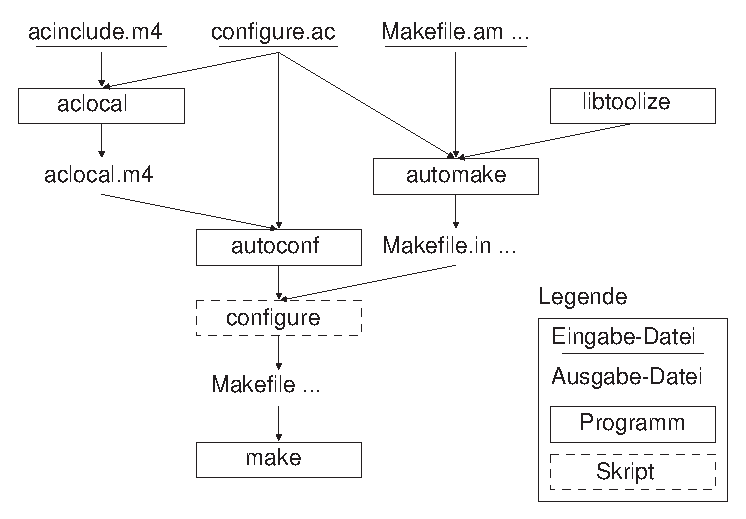
\includegraphics[width=12cm]{Figures/GNUBuildSystem.eps}
  	\caption{GNU build system}
  	\label{fig:GNUBuild}
\end{figure}
The role of the procedures can be summarized as follows.\footnote{in detail: \url{www.gnu.org/software/[autoconf,automake,libtool]/manual}}\par\nopagebreak
	\begin{tabular}{|l|p{100mm}|}
	\hline
		\texttt{aclocal} & Generates M4 macros necessary for the following procedures.\\\hline
		\texttt{autoheader} & Creates \texttt{config.h.in} as basis for header files.\\\hline
		\texttt{autoconf} & Compiler for \texttt{configure.ac} to build the executable \textsc{configure} procedure.\\\hline
		\verb|libtoolize -c --force| & Generates shell and M4 procedures for the system depending shared object files. The option \texttt{-c} forces a local copy of the defining files instead of links. The option \texttt{--force} overwrites already existing procedures.\\\hline
		\texttt{automake -a -c --force} & Compiler for \texttt{Makefile.am} for preparation of \texttt{Makefile.in}. The option \texttt{-c} forces a local copy of the defining files instead of links.\\\hline
		%\verb|./configure| & Substitutes in existing \texttt{.in}-files variables by systemdepending informationen, i.e. paths. With \texttt{CFLAGS}, \texttt{CXXFLAGS}, \texttt{F77FLAGS} and \texttt{FFFLAGS} the compiler can create code for degugging with \texttt{ddd} or \texttt{valgrind} (\texttt{g3}) or for release (\texttt{O2}). The options \verb|--disable-static| accelerates compiling, as the compiler only has to create dynamic (*.so) and no static libraries (*.a). In all source files \texttt{<config.h>} has to be included. \\\hline
		\texttt{make} & Compiles the project sources and links with preliminary libraries. On multi-core computers it is possible to define the number~\texttt{n} of parallel jobs with \texttt{-jn}.\\\hline
		\texttt{make install} & Copies the executable project files and \texttt{includes} to \texttt{MBSim/Install}.\\\hline 
        \texttt{./configure} & Invokes system dependent checks. The option \texttt{--enable-static --disable-shared} only produces a static build, vice versa a shared library is built. Without such an option normally both shared and static libraries are provided.\\\hline
	\end{tabular}
\par It is reasonable to write an executable file invoking the procedures.\\
\par The procedure \textsc{reinstall}
\begin{verbatim}
 ./config.status -recheck
 ./config.status
 make clean
 make install
\end{verbatim}
newly installs a project.\par
For restoring a not-configured version of the project
\begin{verbatim}
 make maintainer-clean
\end{verbatim}
is used. After that \textsc{configure} has to be invoked again.\par 
For uninstall
\begin{verbatim}
 make clean
 make uninstall
\end{verbatim}
has to be called in all directories.

%%------------------------------------------------------------ SUBSUBSECTION --
\subsection{\FMatVec{}}
\FMatVec{} is a library based on LAPack with the possibility to use ATLAS, which is faster for large system dimensions because of internal parallelisation.\\
For the installation the following instructions have to be completed in the directory \texttt{MBSim}. After
\begin{verbatim}
 svn checkout http://svn.berlios.de/svnroot/repos/fmatvec/trunk fmatvec
\end{verbatim}
in the directory \texttt{MBSim/fmatvec} one continues with the procedure \textsc{automake}.\\
Last the procedure \textsc{configure} is used selecting the FLAGS
\begin{verbatim}
 --enable-atlas (use ATLAS)
 --with-blas-lib-prefix=PFX (prefix, where the BLAS lib is
     installed, when ATLAS is not used)
 --with-lapack-lib-prefix=PFX (prefix, where the LAPACK lib is
     installed, when ATLAS is not used)
 --with-atlas-inc-prefix=PFX (prefix, where the ATLAS includes 
     are installed, when ATLAS is used)
 --with-atlas-lib-prefix=PFX (prefix, where the ATLAS libs are
     installed, when ATLAS is used)
\end{verbatim}
if ATLAS should be used instead of LAPack. Details for adapting the installation can be found in \texttt{MBSim/fmatvec/README}. The code can be compiled and installed with the procedure \textsc{install}. For new installations one has to invoke the procedure \textsc{reinstall}.

%%------------------------------------------------------------ SUBSUBSECTION --
\subsection{\HDF}
\HDF can be downloaded from \url{http://www.hdfgroup.org/HDF5/} with at least version 1.8.2. After extracting one uses the procedure \textsc{configure} with the additional FLAG
\begin{verbatim}
 --enable-cxx
\end{verbatim}
and \textsc{install} in the directory \texttt{MBSim/hdf5-1.8.2}.

The \HDF wrapper is available by
\begin{verbatim}
 svn checkout http://svn.berlios.de/svnroot/repos/hdf5serie/trunk HDF5Serie
\end{verbatim}
as well as the procedures \textsc{automake, configure} and \textsc{install} in the directory \texttt{MBSim/HDF5Series}. Last, \texttt{.bashrc} can be extended with
\begin{verbatim}
alias h5lsserie="MBSim/HDF5Serie/hdf5serie/dump/h5lsserie"
alias h5dumpserie="MBSim/HDF5Serie/hdf5serie/dump/h5dumpserie"
\end{verbatim}
to gain overall access to the commands \texttt{h5lsserie} and \texttt{h5dumpserie}.

%%------------------------------------------------------------ SUBSUBSECTION --
\subsection{\OpenMBV{}}
\OpenMBV{} visualises \MBSim{} simulations using XML and HDF5 in a coinciding hierarchical structure. The installation consists of two steps: first \MBSim{} needs \textsf{OpenMBV-C++Interface}, second \OpenMBV{} has to be build for visualisation. The source code is available by
\begin{verbatim}
 svn checkout http://svn.berlios.de/svnroot/repos/openmbv/trunk OpenMBV
\end{verbatim}

\subsubsection{OpenMBV-C++Interface}
The C++-Interface creates standard data for \OpenMBV{} using C++ programs. 
Necessary for its installation are
\begin{itemize}
\item hdf5 with version 1.8.2 or newer (file handling),
\item HDF5Serie (wrapper for file handling).
\end{itemize}
Use the procedures \textsc{automake, configure} and \textsc{install} in \texttt{MBSim/OpenMBV/openmbvcppinterface}. One can find adaptations of this installation process in \texttt{MBSim/OpenMBV/C++Interface/INSTALL}.  For a new installation the procedure \textsc{reinstall} is invoked.

\subsubsection{\OpenMBV{}}
Necessary for the installation of a static visualisation part are the following preliminary steps with everything being installed in \texttt{/home/OpenMBV} and with some hints:
\begin{itemize}
\item \texttt{export PKG\_CONFIG\_PATH=/home/OpenMBV/local/lib/pkgconfig}
\item Coin3d with version 3 or newer (3D scenegraphs)\\
    \texttt{./configure --prefix=/home/OpenMBV/local --disable-shared --enable-static}
\item hdf5 with version 1.8.2 or newer (file handling)\\
    \texttt{./configure --prefix=/home/OpenMBV/local --disable-shared --enable-static\\ --enable-cxx --with-zlib=no}
\item Qt with version 4.4 or newer (2D user interface)\\
    \texttt{./configure -prefix /home/OpenMBV/local -static -nomake examples -nomake demos\\ -nomake docs -nomake translations -no-gif -no-libtiff -qt-libpng -no-libmng\\ -qt-libjpeg -no-openssl -no-glib}
\item HDF5Serie (wrapper for file handling)\\
    \texttt{./configure --prefix=/home/OpenMBV/local --disable-shared --enable-static}
\item SoQt with version 1.5 or newer (e.g. event invocation in coin due to hardware events)\\
    \texttt{in SoQtComponent.cpp:103' change "unsinged long key" to "uintptr\_t key"}\\
    \texttt{export QTDIR=/home/OpenMBV/local}\\
    \texttt{export CONFIG\_QTLIBS="\$(pkg-config --libs QtGui QtCore Qt3Support QtOpenGL)"}\\
    \texttt{./configure --prefix=/home/OpenMBV/local --disable-shared --enable-static}
\item Qwt with version 5 or newer (GUI elements)\\
    \texttt{in qwtconfig.pri change INSTALLBASE=/home/OpenMBV/local}\\
    \texttt{/home/OpenMBV/local/bin/qmake}
\end{itemize}
{\small Fortunately at the institute these steps have already been done at \texttt{diesel:/home/OpenMBV}.}\par
Missing is the final installation. After typing
\begin{verbatim}
export PKG_CONFIG_PATH=/home/OpenMBV/local/lib/pkgconfig:MBSim/Install/lib/pkgconfig
\end{verbatim} 
one should use the procedures \textsc{automake, configure} and \textsc{install} in \texttt{MBSim/OpenMBV/mbxmlutils} for a static build . The procedures \textsc{automake, configure} and \textsc{install} for a static build in \texttt{MBSim/OpenMBV} complete the installation. \texttt{make doc} produces a HTML documentation.\\
There is also a static Linux binary available at \url{www.berlios.de}.\\
Last, \texttt{.bashrc} can be extended with
\begin{verbatim}
 alias openmbv="MBSim/OpenMBV/openmbv/openmbv"
\end{verbatim}
to gain overall access to the command \texttt{openmbv}.

%%------------------------------------------------------------ SUBSUBSECTION --
\subsection{\MBSim}
For installation of \MBSim{} one types
\begin{verbatim}
 svn checkout http://svn.berlios.de/svnroot/repos/mbsim/trunk mbsim
\end{verbatim}
in \texttt{MBSim}. Then in single subdirectories the \texttt{kernel}, some \texttt{examples} and some \texttt{modules} are extracted.\\
The file \texttt{.bashrc} has to be extended with
\begin{verbatim}
 export PKG_CONFIG_PATH=
        "MBSim/Install/lib/pkgconfig/:$PKG_CONFIG_PATH"
 export LD_LIBRARY_PATH=
        "MBSim/Install/lib/:$LD_LIBRARY_PATH"
\end{verbatim}
Then the shell has to be restarted or the command \texttt{source .bashrc} is necessary.\\
Now, one invokes the procedures \textsc{automake, configure} and \textsc{install} in the directory \texttt{MBsim/mbsim/kernel}. For a new installation the procedure \textsc{reinstall} is used. \texttt{make doc} creates a HTML documentation. The installation of the modules is analogously.

%%------------------------------------------------------------ SUBSUBSECTION --
\subsection{MBSimAddOns}
{\small At the institute further modules can be found in \texttt{MBSimAddOn}: mechanical components~(\texttt{mbsimMechAdd}), hydraulic components~(\texttt{mbsimHydraulics}), an interface for co-simulationen~(\texttt{mbsimCosim}) and a XML parser~(\texttt{mbsimXML}). For installation one types
\begin{verbatim}
 svn checkout http://zeiss/repos/SVN--rep//AM-software/mbsimAddOn/trunk mbsimAddOn
\end{verbatim}
in directory \texttt{MBSim}. Then one uses the procedures \textsc{automake, configure} and \textsc{install} in the subdirectories of \texttt{MBsim/mbsimAddOn}.
}

%%------------------------------------------------------------ SUBSUBSECTION --
\subsection{\MBSim Examples}
The examples are used for testing successful installation. There are two possibilities:
\begin{enumerate}
\item Change to the specific directory and type \texttt{make} to create an executable. the simulation starts with the command~\texttt{./main}. The results are visualised with the command~\texttt{openmbv} and plotted with the commands from Sec.~\ref{sec:plot}.
\item Use the script \texttt{./runexamples.sh} in the upmost examples directory even to compare with reference data. See \texttt{./runexamples.sh -h} for the syntax. The \HDF{} executables must be available in the search path. For all examples there should exist reference data, which also can be newly uploaded to \url{www.berlios.de} using the \texttt{Admin} button, anonymos ftp-upload, deleting the old file and adding the new one.
\end{enumerate}
